\documentclass{article}
\usepackage{amsmath}
\usepackage{blindtext}
\usepackage[utf8]{inputenc}
\usepackage{amssymb}
\usepackage{setspace}
\usepackage{graphicx}
\usepackage{geometry}
\usepackage{listings}
\usepackage{float}
\usepackage{multicol}
\geometry{left = 1in, right =1in,top=1in, bottom = 1in}
\doublespacing
\begin{document}
\newcommand*{\be}{\mathbb{E}}
\newcommand*{\bv}{\mathbb{V}}
\lstset{showspaces = false, showstringspaces = false}
\linespread{2}
\title{Numerical Comparative Dynamics: Ball Python Breeding}
\author{Donald DiJacklin}
\maketitle
\section*{Introduction}
	\indent\indent Selective breeding is performed on many species, whether it's done to increase the size of the offspring, increase the speed of the offspring, or simply make healthier offspring. All of the preceding reasons are done in an effort to make the offspring worth more. In the case of Ball Pythons, the selective breeding is done (most of the time) in an effort to increase the number of visually expressed genes, and among those to express rare genes.\\
	\indent Ball Pythons (\textit{python regius}) are indigenous to Africa, but in recent years have been imported to other countries and seen some success as exotic pets. As in the case of dogs, some people prefer different trtraits to be expressed in a Ball Python. Ball Pythons can have traits that affect colors or patterns or both. As an example, shown below on the left is a Ball Python that looks like most of the Ball Pythons in Africa do called a Normal by snake breeders. On the right is a Ball Python that expresses the trait known as Pastel.
	\begin{multicols}{2}
	\begin{figure}[H]
	\centering
	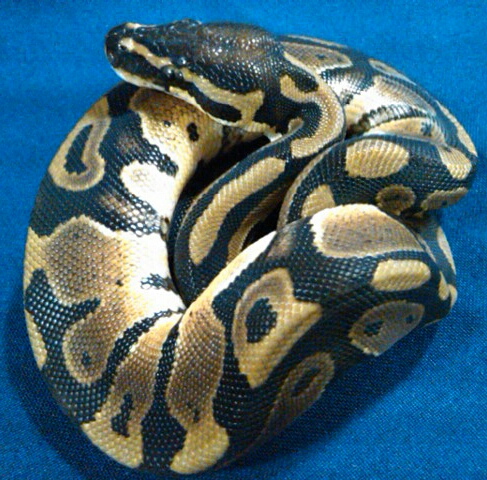
\includegraphics[width=.5\textwidth, height = 62mm]{Normal.jpg}
	\end{figure}
	\begin{figure}[H]
	\centering
	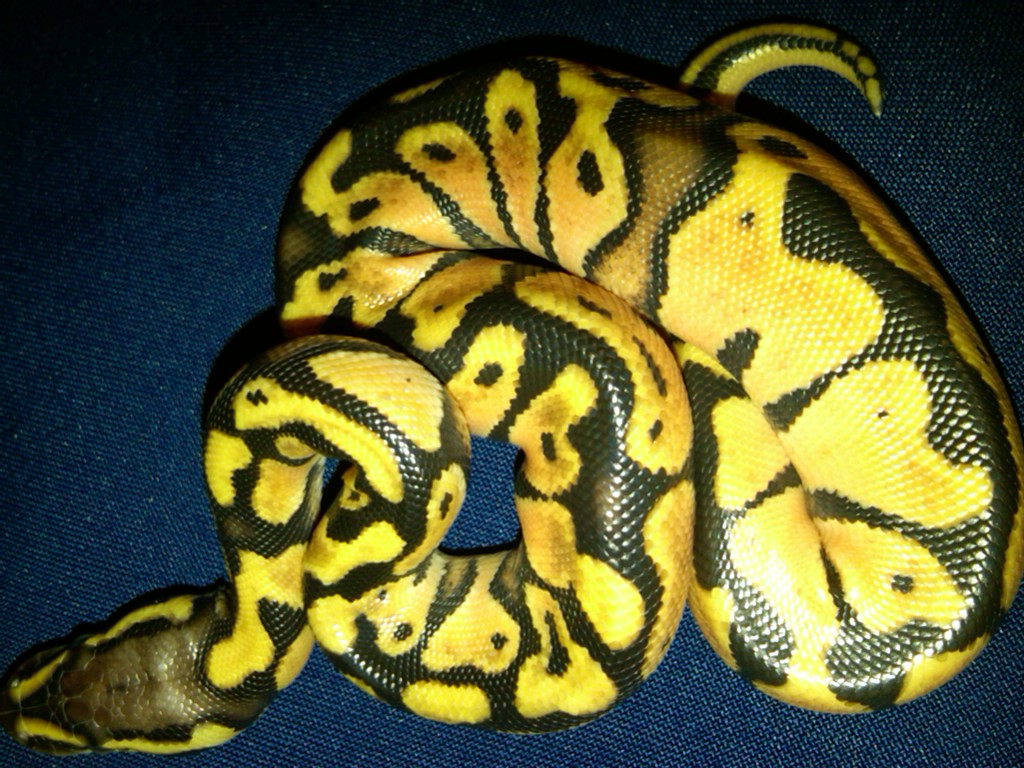
\includegraphics[width=.5\textwidth]{Pastel.jpg}
	\end{figure}
	\end{multicols}
	Note the marked difference that one trait can make in the appearance of the snake. As with dogs, certain traits are valued much higher than others. A Normal costs about \$20, whereas a Pastel costs about \$45, and Ball Python with another trait, called Banana, costs about \$200. As one might imagine the `cooler' looking the snake the more it will cost, so breeders seek to make more money by breeding so offspring will express more genes and therefore look `cooler'.\\
	\indent I will not go over the details of snake reproduction here, but there are certain facts that will be used in this paper and the related programs, without which the reader will undoubtedly be lost. Firstly, upon a successful (and sometimes unsuccesful) pairing of a male and female snake a set of eggs, called a clutch, is produced. Secondly, female snakes can breed up to once per breeding season, whereas a male can breed up to five times per breeding season.

\end{document}